%%%%%%%%%%%%%%%%%%%%%%%%%%%%%%%%%%%%%%%%%
% Journal Article
% LaTeX Template
% Version 1.4 (15/5/16)
%
% This template has been downloaded from:
% http://www.LaTeXTemplates.com
%
% Original author:
% Frits Wenneker (http://www.howtotex.com) with extensive modifications by
% Vel (vel@LaTeXTemplates.com)
%
% License:
% CC BY-NC-SA 3.0 (http://creativecommons.org/licenses/by-nc-sa/3.0/)
%
%%%%%%%%%%%%%%%%%%%%%%%%%%%%%%%%%%%%%%%%%

%----------------------------------------------------------------------------------------
%	PACKAGES AND OTHER DOCUMENT CONFIGURATIONS
%----------------------------------------------------------------------------------------

\documentclass[twoside,twocolumn]{article}

\usepackage[sc]{mathpazo} % Use the Palatino font
\usepackage[T1]{fontenc} % Use 8-bit encoding that has 256 glyphs
\linespread{1.05} % Line spacing - Palatino needs more space between lines
\usepackage{microtype} % Slightly tweak font spacing for aesthetics

\usepackage[english]{babel} % Language hyphenation and typographical rules

\usepackage[hmarginratio=1:1,top=32mm,columnsep=20pt]{geometry} % Document margins
\usepackage[hang, small,labelfont=bf,up,textfont=it,up]{caption} % Custom captions under/above floats in tables or figures
\usepackage{booktabs} % Horizontal rules in tables

\usepackage{lettrine} % The lettrine is the first enlarged letter at the beginning of the text

\usepackage{enumitem} % Customized lists

\usepackage{abstract} % Allows abstract customization
\renewcommand{\abstractnamefont}{\normalfont\bfseries} % Set the "Abstract" text to bold
\renewcommand{\abstracttextfont}{\normalfont\small\itshape} % Set the abstract itself to small italic text

\usepackage{titlesec} % Allows customization of titles
\renewcommand\thesection{\Roman{section}} % Roman numerals for the sections
\renewcommand\thesubsection{\roman{subsection}} % roman numerals for subsections


\usepackage{fancyhdr} % Headers and footers
\pagestyle{fancy} % All pages have headers and footers
\fancyhead{} % Blank out the default header
\fancyfoot{} % Blank out the default footer
\fancyhead[C]{Analysis of Gravitation $\bullet$ May 2017} % Custom header text
\fancyfoot[RO,LE]{\thepage} % Custom footer text

\usepackage{titling} % Customizing the title section

\usepackage{hyperref} % For hyperlinks in the PDF

\usepackage{graphicx}
\usepackage{float}
\usepackage{amsmath}
\usepackage{empheq}

\graphicspath{ {graphics/} }

%----------------------------------------------------------------------------------------
%	TITLE SECTION
%----------------------------------------------------------------------------------------

\title{Analysis of Gravitation: Measuring the Gravitational Constant G} % Article title
\author{
\textsc{Gabriel Smadi} \\ % Your name
\normalsize{Syracuse University} \\ % Your institution
\normalsize \href{mailto:gsmadi@syr.edu}{gsmadi@syr.edu} % Your email address
}

\date{\today} % Leave empty to omit a date

%----------------------------------------------------------------------------------------

\begin{document}

% Print the title
\maketitle

\begin{abstract}
  Abstract here....
\end{abstract}

%----------------------------------------------------------------------------------------
%	ARTICLE CONTENTS
%----------------------------------------------------------------------------------------

\section{Introduction}

Intro here...

%------------------------------------------------

\section{Methods}

\begin{figure}[H]
\centering
  \begin{center}
    \scalebox{.3}{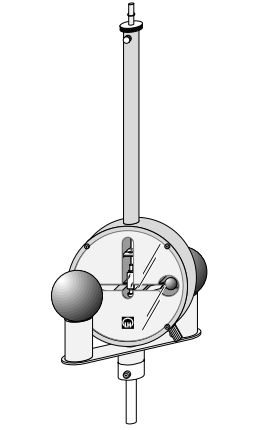
\includegraphics{apparatus}}
  \end{center}
  \caption{Data points and fit function for Position I data}
\end{figure}
\label{fig:apparatus}

\begin{figure}[H]
\centering
  \begin{center}
    \scalebox{.4}{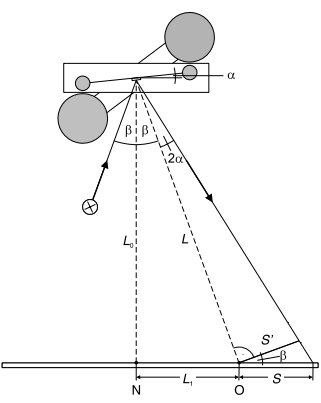
\includegraphics{geometry}}
  \end{center}
  \caption{Data points and fit function for Position I data}
\end{figure}
\label{fig:geometry}

\begin{equation}
\label{eq:attraction}
F = G \mult \frac{m_{1}m_{2}}{r^2}
\end{equation}

\begin{equation}
\label{eq:torque}
\tau_{I} = F_{net} \times r = (2F) \mult d = 2G \mult \frac{m_{1}m_{2}d}{b^2}
\end{equation}

\begin{equation}
\label{eq:pos_torque}
\tau_{I} = -\tau_{II} = \kappa \theta
\end{equation}

\begin{equation}
\label{eq:diff_eq}
  I\frac{d^2\theta}{dt^2} + D\frac{d\theta}{dt} + \kappa \theta = 0
\end{equation}

where $\kappa$ is the torsion constant and D the damping factor.

\begin{equation}
\label{eq:diff_sol}
\theta(t) = \theta_{0}cos(\omega t + \phi)e^{-\frac{t}{\tau}} + C
\end{equation}

where $\tau = 1 / \kappa $

\begin{equation}
\label{eq:period}
T = 2\pi \mult \sqrt{\frac{I}{\kappa}}
\end{equation}

For a rigid rod the moment of inertia is given by,

\begin{equation}
\label{eq:inertia}
I = m_{2}(\frac{d}{2})^2 + m_{2}(\frac{d}{2})^2 = \frac{m_{2}d^2}{2}
\end{equation}

\begin{equation}
\label{eq:kappa}
\kappa = \frac{2m_{2}d^2\pi^2}{T^2}
\end{equation}

Let $\theta = (\alpha_{I} - \alpha_{II})$, which is ...

The net torque ...

\begin{equation}
\label{eq:net_roque}
\tau_{net} = Fd = \kappa\theta = \kappa(\alpha_{I} - \alpha_{II})
\end{equation}

$\Rightarrow$
$$
  (\frac{Gm_{1}m_{2}}{b^2}) \mult d = \kappa (\alpha_{I} - \alpha_{II})
$$

$\Rightarrow$
$$
  (\frac{Gm_{1}m_{2}}{b^2}) \mult d = (\frac{2m_{2}d^2\pi^2}{T^2}) \mult (\alpha_{I} - \alpha_{II})
$$

$\Rightarrow$

\begin{equation}
\label{eq:almost_g}
G = \frac{2\pi^{2}db^2}{m_{1}T^2} \mult (\alpha_{I} - \alpha_{II})
\end{equation}

By inspection of the configuration geometry we find that,

$$
  \alpha_{I} = \frac{S_{I}}{2} \mult \frac{L_{0}}{L_{0}^2 + L_{1}^2}, \quad
  \alpha_{II} = \frac{S_{II}}{2} \mult \frac{L_{0}}{L_{0}^2 + L_{1}^2}
$$

$\Rightarrow$

\begin{equation}
\label{eq:delta_alpha}
  (\alpha_{I} - \alpha_{II}) = \frac{(S_{I} - S_{II})}{2} \mult \frac{L_{0}}{L_{0}^2 + L_{1}^2}}
\end{equation}

Therefore, by Eq. \ref{eq:almost_g} and Eq. \ref{eq:delta_alpha} our final equations for G is,

\begin{equation}
\label{eq:final_g}
  \boxed{G = \frac{\pi^{2}b^2d}{m_{1}} \mult \frac{(S_{I} - S_{II})}{T^2} \mult \frac{L_{0}}{L_{0}^2 + L_{1}^2}}
\end{equation}


Text requiring further explanation\footnote{Example footnote}.

%------------------------------------------------

\section{Results}


\begin{figure}[H]
\centering
  \begin{center}
    \scalebox{.5}{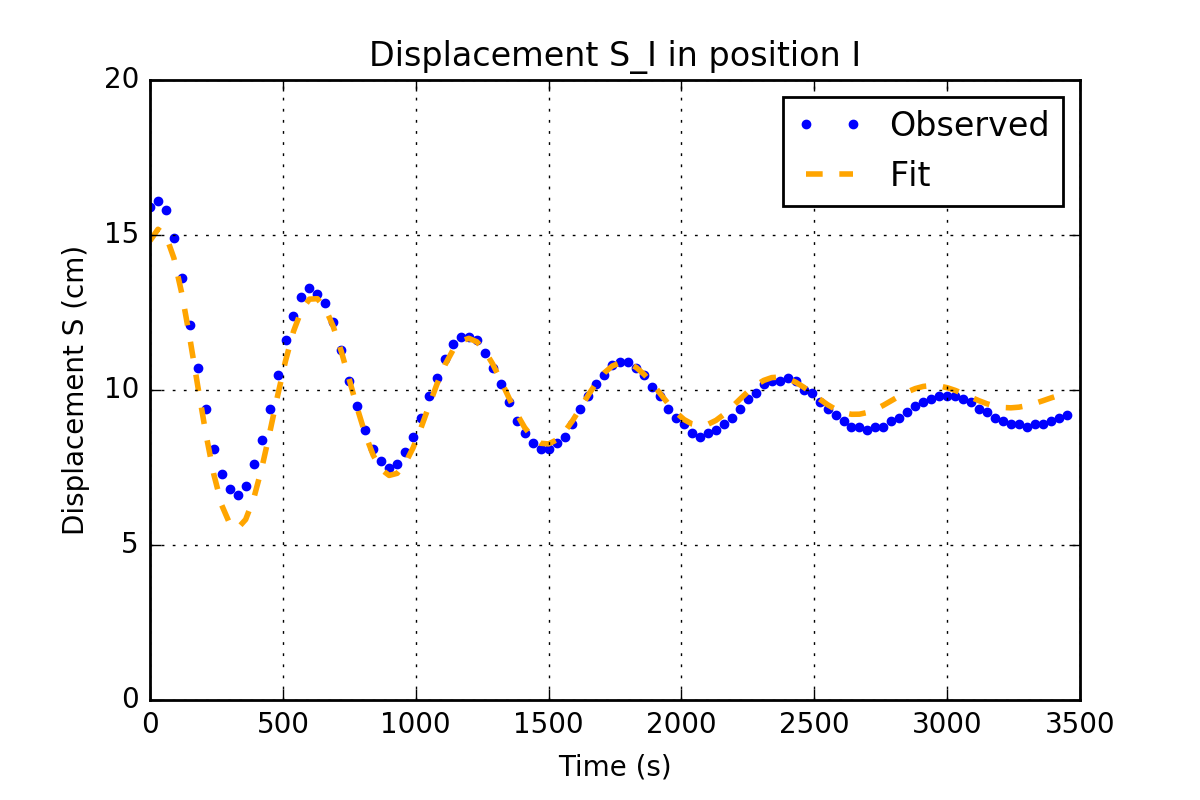
\includegraphics{pos1_datafit}}
  \end{center}
  \caption{Data points and fit function for Position I data}
\end{figure}
\label{fig:pos1_plot}

\begin{table}[H]
\caption{Optimized fit function parameters for Position I}
\centering
\begin{tabular}{llr}
\toprule
\cmidrule(r){1-2}
Parameter & Value \\
\midrule
$ A$ & $ 5.6 \pm 0.2 $ \\
$ \tau$ & $ 1120 \pm 61 $ \\
$ T$ & $ 582 \pm 3 $ \\
$ \phi$ & $ -0.45 \pm 0.04 $ \\
$ C$ & $ 9.74 \pm 0.04 $ \\
\bottomrule
\end{tabular}
\end{table}

\begin{figure}[H]
\centering
  \begin{center}
    \scalebox{.5}{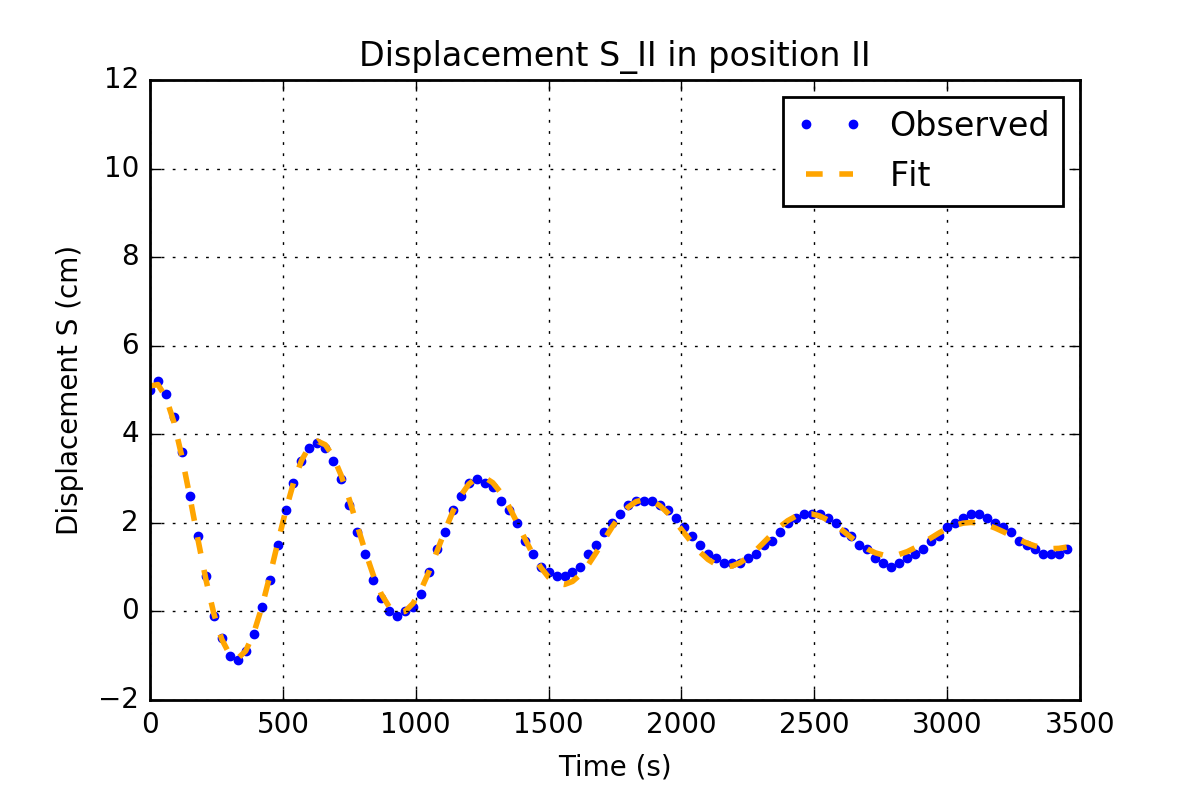
\includegraphics{pos2_datafit}}
  \end{center}
  \caption{Data points and fit function for Position II data}
\end{figure}
\label{fig:pos2_plot}

\begin{table}[H]
\caption{Optimized fit function parameters for Position II}
\centering
\begin{tabular}{llr}
\toprule
\cmidrule(r){1-2}
Parameter & Value \\
\midrule
$ A$ & $ 5.53 \pm 0.04 $ \\
$ \tau$ & $ 1307 \pm 24 $ \\
$ T$ & $ 614.6 \pm 0.9 $ \\
$ \phi$ & $ -0.26 \pm 0.013 $ \\
$ C$ & $ 1.68 \pm 0.9 $ \\
\bottomrule
\end{tabular}
\end{table}

%------------------------------------------------
\section{Analysis}

\begin{table}[H]
\caption{Summary of measurements}
\centering
\begin{tabular}{llr}
\toprule
\cmidrule(r){1-2}
Parameter & Value \\
\midrule
$\ L_{0}$ & $ 5.53 \pm 0.04 $ m \\
$\ L_{1}$ & $ 1307 \pm 24 $ cm \\
$\ S_{I}$ & $ 614.6 \pm 0.9 $ cm \\
$\ S_{II}$ & $ -0.26 \pm 0.013 $ cm \\
$\ T$ & $ 1.68 \pm 0.9 $ s \\
\bottomrule
\end{tabular}
\end{table}


\begin{equation}
\label{eq:error}
 \% error = \frac{\abs{G_{measured} - G}}{G} \mult 100
\end{equation}

%------------------------------------------------

\section{Discussion}

\subsection{Subsection One}

A statement requiring citation \cite{Figueredo:2009dg}.


\subsection{Subsection Two}

%----------------------------------------------------------------------------------------
%	REFERENCE LIST
%----------------------------------------------------------------------------------------

\begin{thebibliography}{99} % Bibliography - this is intentionally simple in this template

\bibitem[Figueredo and Wolf, 2009]{Figueredo:2009dg}
Figueredo, A.~J. and Wolf, P. S.~A. (2009).
\newblock Assortative pairing and life history strategy - a cross-cultural
  study.
\newblock {\em Human Nature}, 20:317--330.

\end{thebibliography}

%----------------------------------------------------------------------------------------

\end{document}
